\clearpage
\section{Impact parameter \label{sec:impactparameter}}
The impact parameter (IP) is defined as the minimum distance between
the primary vertex and the trajectory of the track. Tracks produced by
long lived particles such as B mesons are expected to have a sizable
IP.  In the ultra-relativistic limit the IP is Lorentz-invariant to a
good approximation due to the cancellation of boost effects and the
angle of the decay products with respect to the flight path. The
precision of the IP measurement can be different from track to track
and is between 30~$\mu$m and several hundreds $\mu$m. Given that the
uncertainty can be of the same order as the IP value, the IP
significance $S= IP/\sigma_{IP}$ is used for tagging b-jets. 

The IP is ``lifetime signed'': tracks originating from the decay of
particles traveling in the same direction of the jet are signed as
positive, while those in opposite direction are tagged as
negative. This is obtained by using the sign of the scalar product of
the IP segment with the jet direction. It should be noted that a ``sign
flip'' can happen to track produced in the region between the jet
direction and the actual B-hadron flight direction. 


The IP can be measured either in the transverse plane only or in three
dimensions. The high resolution of the pixel detector also along the z
coordinate allows the use of the 3D IP: despite the precision in z being slightly inferior with respect to the one in the
transverse plane, by using the 3D significance the precision is not 
spoiled as the measurement errors are correctly taken into account.   
 

3D Impact Parameter value, error and significance for first, second and
third track in the jet (ordered by IP significance) are displayed in
Figures~\ref{fig:IPfirstTrack} to \ref{fig:IPThirdTrack}. Figure
\ref{fig:IPAllTrack} shows the same for all selected tracks in a jet
(i.e. not ordered by IP significance).

\begin{figure}[h!]
\centering
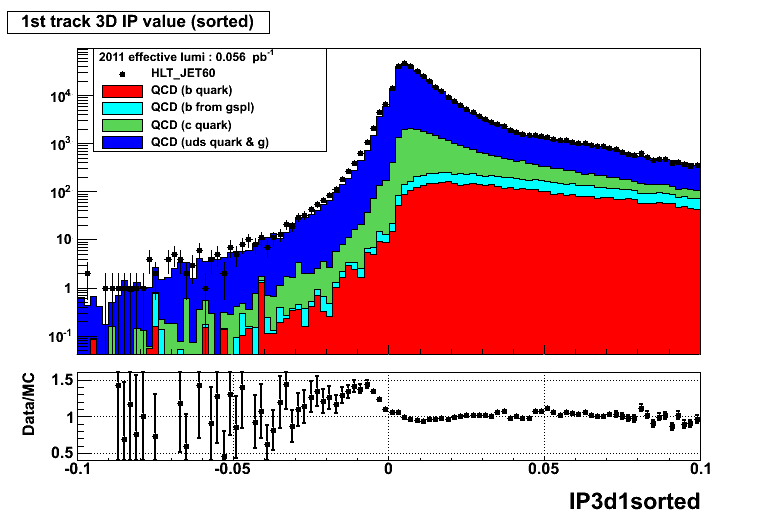
\includegraphics[width=0.32\textwidth]{figures/IP3d1sorted_Log.png}
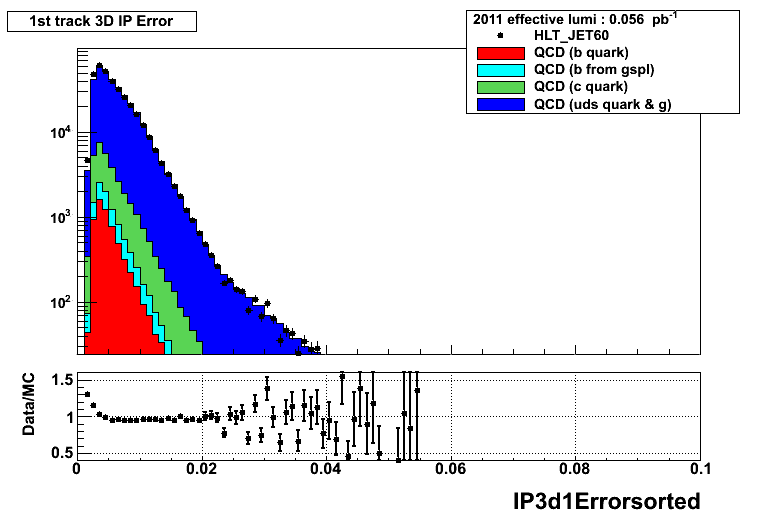
\includegraphics[width=0.32\textwidth]{figures/IP3d1Errorsorted_Log.png}
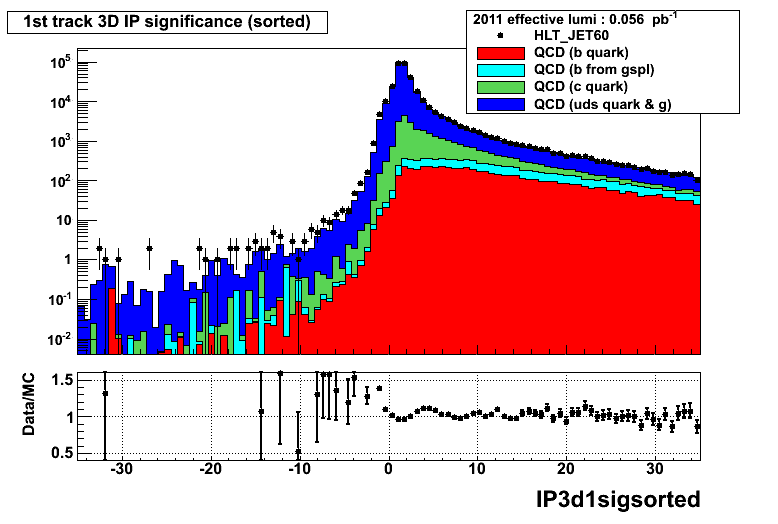
\includegraphics[width=0.32\textwidth]{figures/IP3d1sigsorted_Log.png}
\caption{Left: IP value, middle: IP error, right: IP significance for the first track in the jet, ordered by IP significance.  }
\label{fig:IPfirstTrack}
\end{figure}

\begin{figure}[h!]
\centering
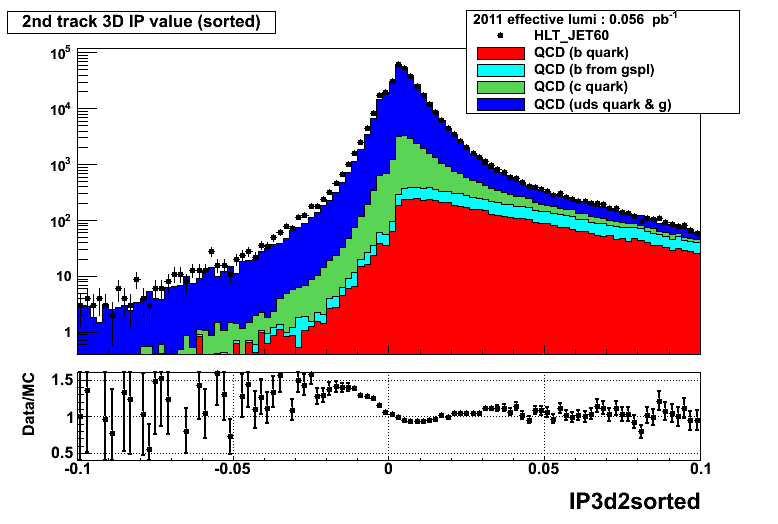
\includegraphics[width=0.32\textwidth]{figures/IP3d2sorted_Log.png}
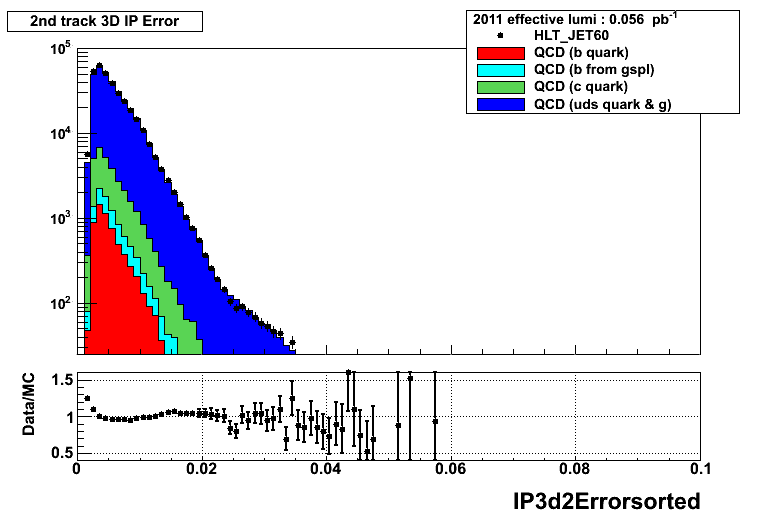
\includegraphics[width=0.32\textwidth]{figures/IP3d2Errorsorted_Log.png}
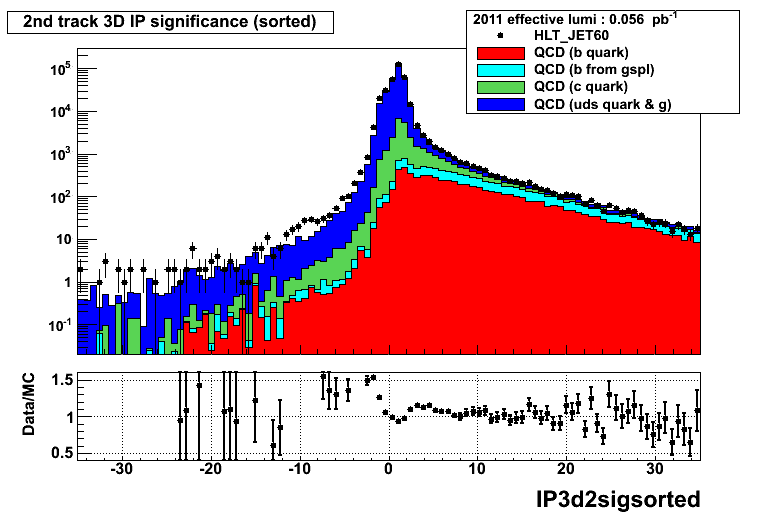
\includegraphics[width=0.32\textwidth]{figures/IP3d2sigsorted_Log.png}
\caption{Left: IP value, middle: IP error, right: IP significance for the second track in the jet, ordered by IP significance.  }
\label{fig:IPsecondTrack}
\end{figure}

\begin{figure}[h!]
\centering
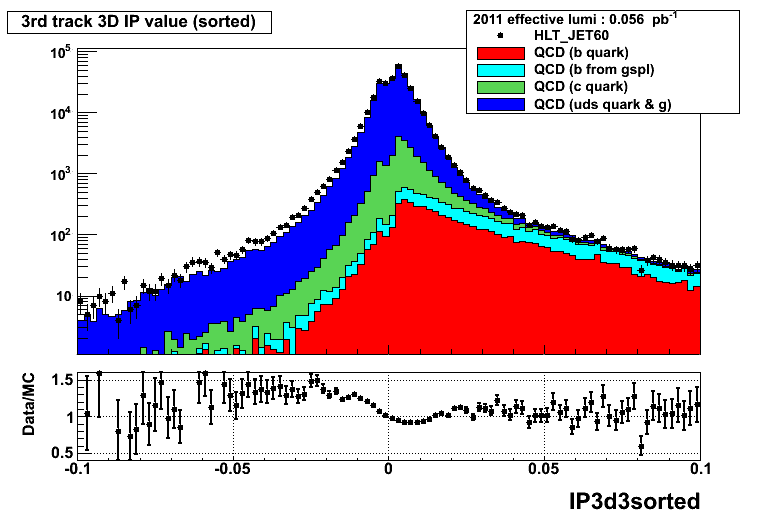
\includegraphics[width=0.32\textwidth]{figures/IP3d3sorted_Log.png}
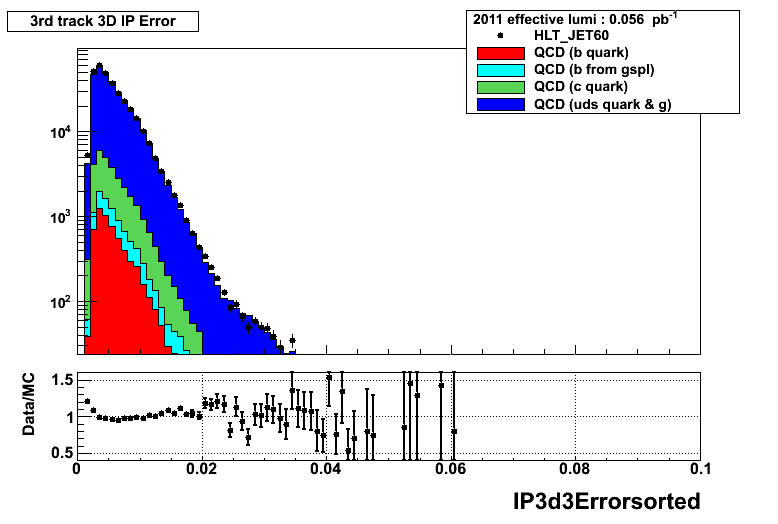
\includegraphics[width=0.32\textwidth]{figures/IP3d3Errorsorted_Log.png}
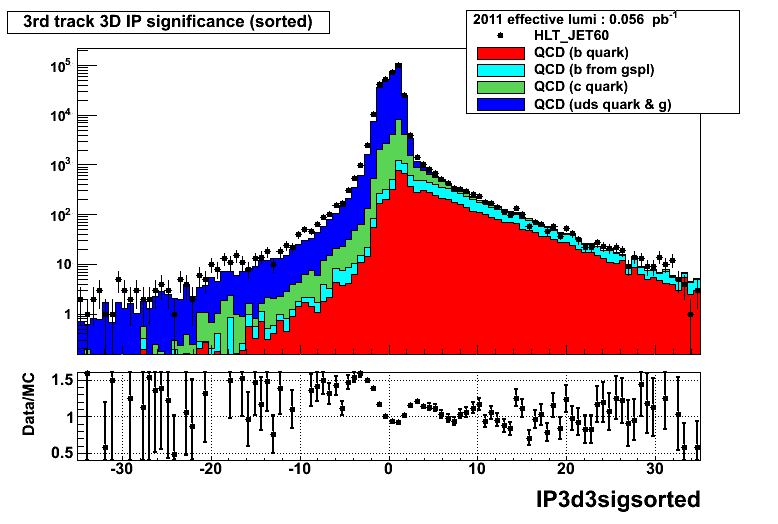
\includegraphics[width=0.32\textwidth]{figures/IP3d3sigsorted_Log.png}
\caption{Left: IP value, middle: IP error, right: IP significance for the third track in the jet, ordered by IP significance.  }
\label{fig:IPThirdTrack}
\end{figure}

\begin{figure}[h!]
\centering
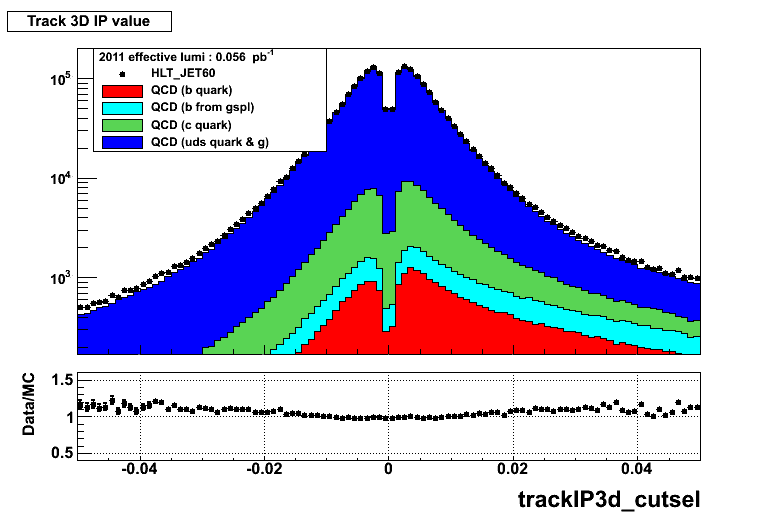
\includegraphics[width=0.32\textwidth]{figures/trackIP3d_cutsel_Log.png}
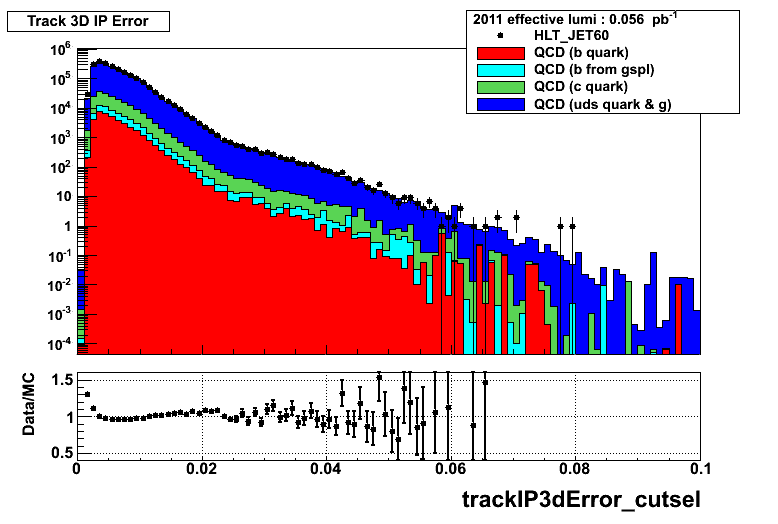
\includegraphics[width=0.32\textwidth]{figures/trackIP3dError_cutsel_Log.png}
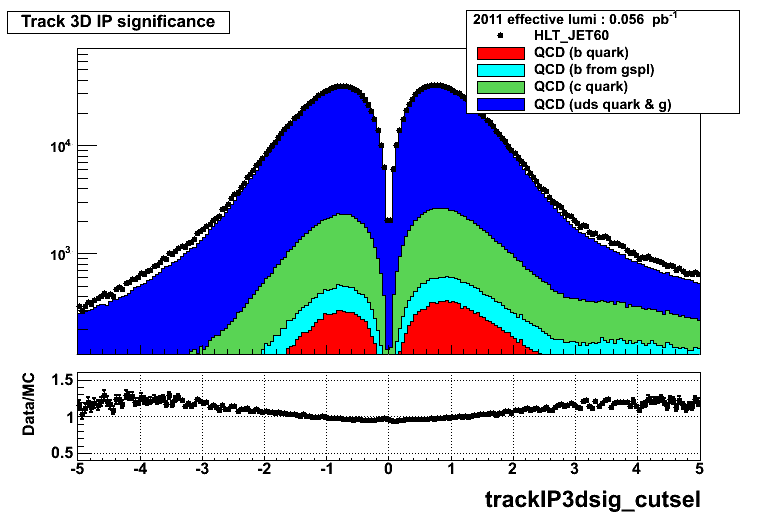
\includegraphics[width=0.32\textwidth]{figures/trackIP3dsig_cutsel_Log.png}
\caption{Left: IP value, middle: IP error, right: IP significance for all selected tracks in the jet. The track selection as defined in Section~\ref{sec:trackselection} has been applied.}
\label{fig:IPAllTrack}
\end{figure}



The impact parameter has slightly different behaviour depending on the track momentum. This is shown in Figure~\ref{fig:IPbinnedTrackpt} which displays the track IP values for six different track $p_t$ bins.  

% A major source of discrepancies is the number of tracks associated to the jets. This is visible in Figure~\ref{fig:IPBinnedInNtracks} which shows the first track $p_t$ bin split into nince bins of number of tracks per jet.



\begin{figure}[h!]
\centering
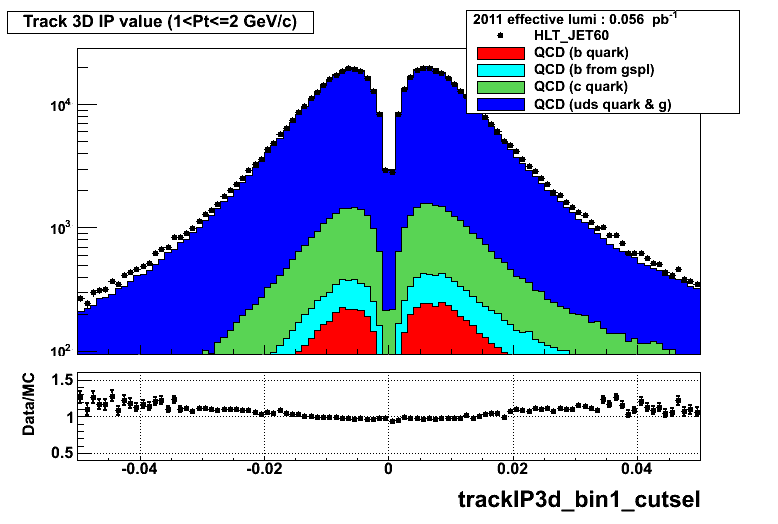
\includegraphics[width=0.32\textwidth]{figures/trackIP3d_bin1_cutsel_Log.png}
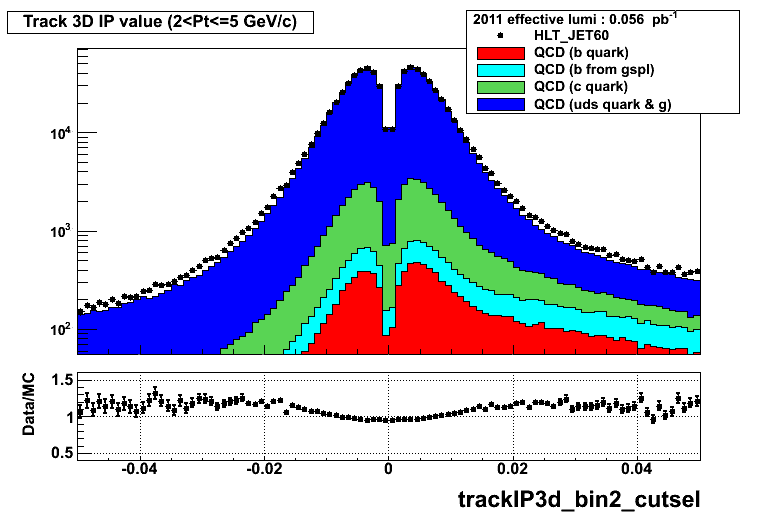
\includegraphics[width=0.32\textwidth]{figures/trackIP3d_bin2_cutsel_Log.png}
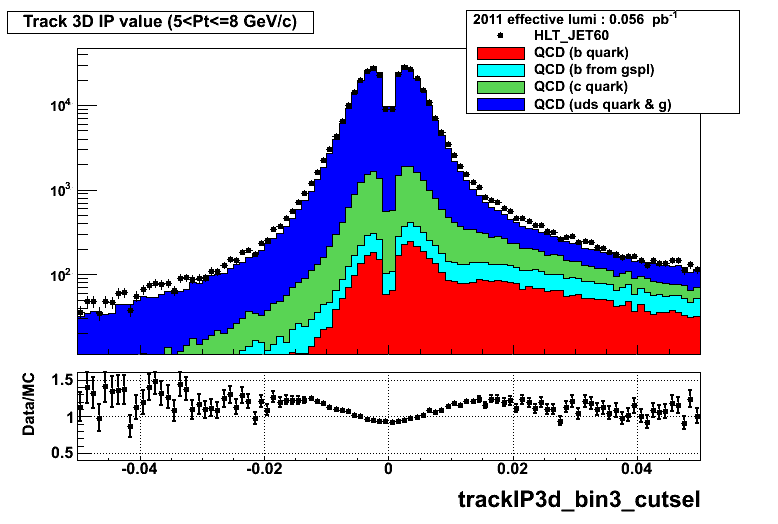
\includegraphics[width=0.32\textwidth]{figures/trackIP3d_bin3_cutsel_Log.png}
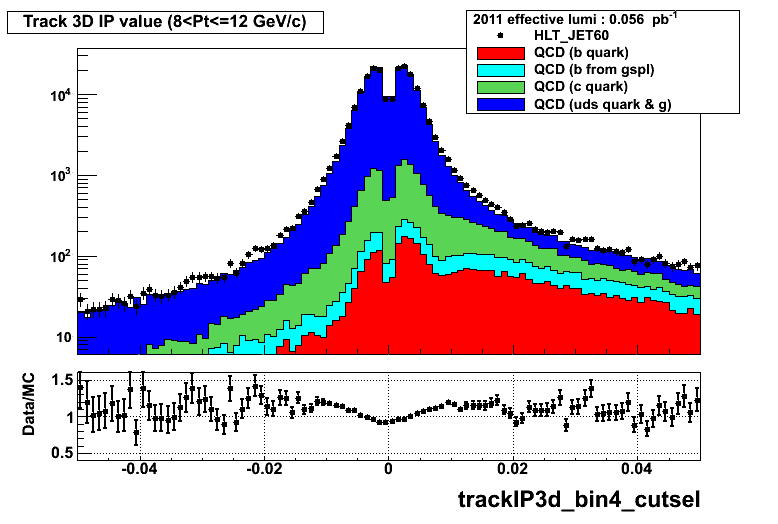
\includegraphics[width=0.32\textwidth]{figures/trackIP3d_bin4_cutsel_Log.png}
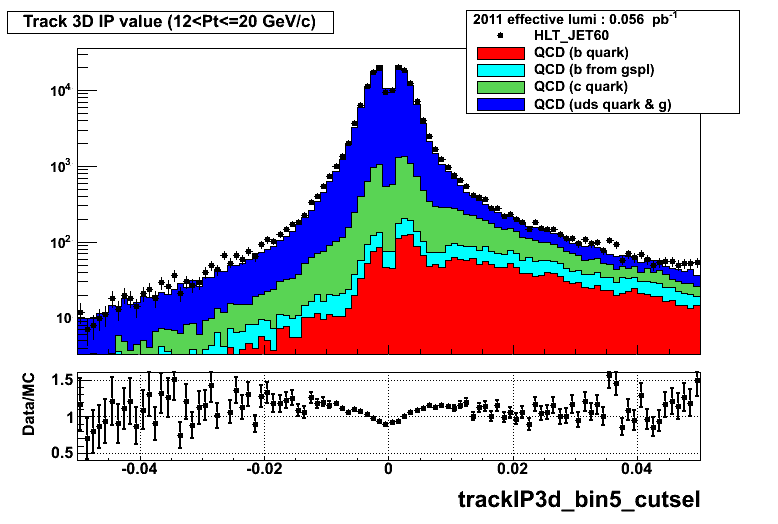
\includegraphics[width=0.32\textwidth]{figures/trackIP3d_bin5_cutsel_Log.png}
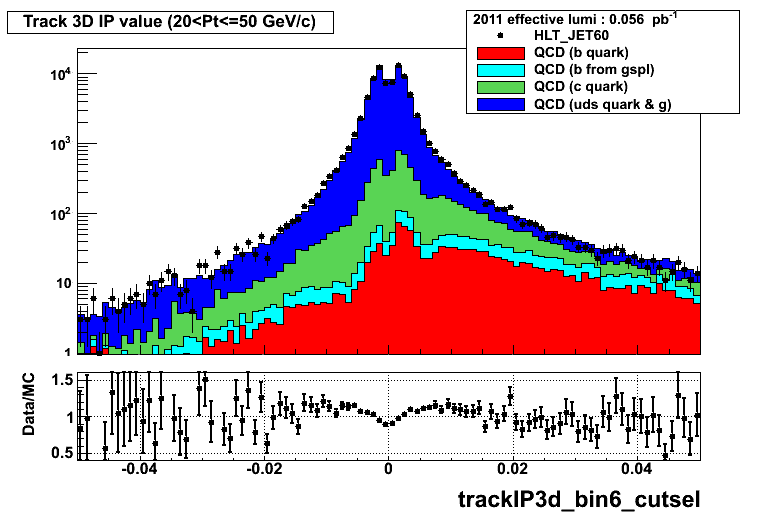
\includegraphics[width=0.32\textwidth]{figures/trackIP3d_bin6_cutsel_Log.png}
\caption{The IP value in six bins of track $p_t$. From top left to bottom right (in units of GeV/$c$): $1<p_t<2; \ 2<p_t<5; \ 5<p_t<8; \ 8<p_t<12; \ 12<p_t<20; \ 20<p_t<50$.   }
\label{fig:IPbinnedTrackpt}
\end{figure}

